\chapter*{Proposition 15}
\label{prop:15}

\begin{figure*}[ht]
    \begin{center}
    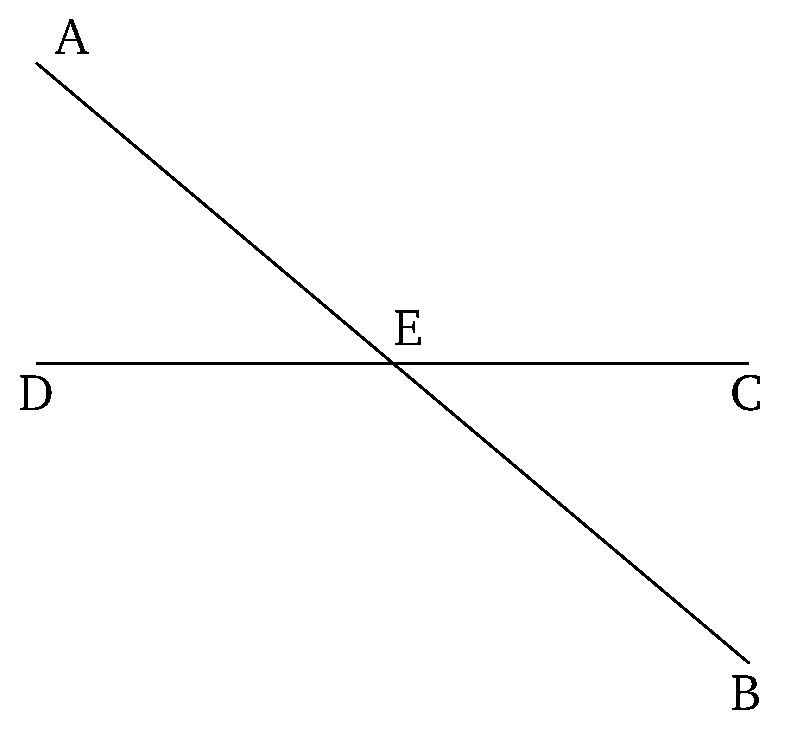
\includegraphics[width=0.5\linewidth]{figures/fig15e.eps}
    \label{fig:prop_15}
    \end{center}
\end{figure*}

If two straight-lines cut one another then they make the vertically opposite angles
equal to one another.

For let the two straight-lines $AB$ and $CD$ cut one another at the point $E$. I say
that  angle $AEC$ is equal to (angle) $DEB$, and (angle) $CEB$ to (angle) $AED$.

For since the straight-line $AE$ stands on the straight-line $CD$, making the
angles $CEA$ and $AED$, the (sum of the) angles $CEA$ and $AED$ is thus equal to two
right-angles [Prop.~1.13]. Again, since the straight-line $DE$ stands on the
straight-line $AB$, making the angles $AED$ and $DEB$, the (sum of the) angles $AED$ and
$DEB$ is thus equal to two right-angles [Prop.~1.13]. But (the sum of) $CEA$ and $AED$ was also shown
(to be) equal to two right-angles. Thus, (the sum of) $CEA$ and $AED$ is equal to (the sum of) $AED$ and $DEB$ [C.N.~\ref{cn:1}]. Let $AED$ have been subtracted from both. Thus, the remainder
$CEA$ is equal to the remainder $BED$ [C.N.~\ref{cn:3}]. Similarly, it can be shown that
$CEB$ and $DEA$ are also equal.

Thus, if two straight-lines cut one another then they make the vertically opposite angles
equal to one another. (Which is) the very thing it was required to show.


\section*{Commentary}

\begin{proposition}\label{proposition_15}\lean{Elements.Book1.proposition_15}\leanok
    $AB$ and $CD$ are two different lines intersecting at $E$. $A$ and $B$ are two distinct points on $AB$. $C$ and $D$ are two distinct points on $CD$. $E$ is between $A$ and $B$, and $E$ is also between $C$ and $D$. Then, we have $\angle~AEC = \angle~DEB$ and $\angle~CEB = \angle~AED$.
\end{proposition}
\begin{proof}
    \uses{proposition_13}\leanok
    See the original proof by Euclid.
\end{proof}
